\documentclass[addpoints,12pt]{exam}


\makeatletter
\expandafter\providecommand\expandafter*\csname ver@framed.sty\endcsname
{2003/07/21 v0.8a Simulated by exam}
\makeatother

\usepackage{xcolor}
\usepackage{minted}
\usepackage[utf8]{inputenc}
\usepackage{tikz}
\usepackage{caption}
\usepackage{gensymb}
\usepackage{lmodern}
\usepackage{multirow}
\usepackage{booktabs}
\usepackage{array}
\usepackage{adjustbox}
\usepackage{upquote}
\usepackage{amsmath}
\usepackage[hidelinks]{hyperref}
\usetikzlibrary{mindmap,shadows, shapes, arrows, positioning}

\tikzstyle{rect} = [rectangle, fill=ProcessBlue, text width=4.5em, text centered, minimum height=4em, rounded corners]
\tikzstyle{line} = [draw, ->, very thick]
\tikzstyle{oval} = [ellipse, fill=SeaGreen, text width=5em, text centered]

\newcolumntype{x}[1]{>{\centering\arraybackslash\hspace{0pt}}p{#1}}

\renewcommand{\refname}{\selectfont\normalsize References} 
\pagestyle{headandfoot}

\header{\textbf{Problem Sheet: Seven Bridges of Königsberg}}{}{Graph Theory}
\footer{}{Page \thepage\ of \numpages}{}
\marksnotpoints
\pointsinrightmargin

\begin{coverpages}
\end{coverpages}

\begin{document}

\noindent
The following problem was first presented by Leonhard Euler~\cite{euleroriginal}.
The problem concerns a former city called Königsberg, which is now called Kaliningrad, in Prussia (now in Russia).
Take the time to try to solve this problem yourself.

\subsubsection*{Question}
In Königsberg, there were seven bridges linking four different parts of the city.
These are depicted in the diagram below.
The question is: is it possible to walk through the city crossing each bridge once and only once~\cite{konigsbergwikipedia}?

\begin{center}
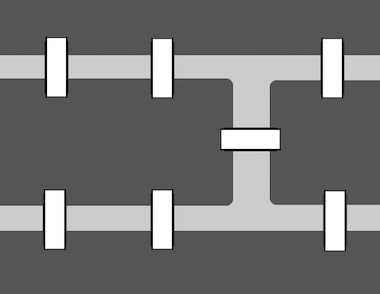
\includegraphics{diagram}
\end{center}


\bibliographystyle{plain}
\bibliography{bibliography}
\end{document}
